\documentclass[11pt, openright]{book}

    % Cover Variables
    \newcommand{\ctoptitle}{THEORY OF }
    \newcommand{\ctitle}{FIBER BRAGG GRATINGS}
    \newcommand{\cautor}{Lucas}
    \newcommand{\cdate}{day.month.year}
    \newcommand{\sectittle}{Thoery of Fiber Bragg Gratings}


    % Header Variables
        \newcommand{\headRE}{Theory of Fiber Bragg gratings}
        \newcommand{\headLE}{\emph{\rightmark}}
        \newcommand{\footRE}{Lucas Lescure $-$ \cdate}
        \newcommand{\footLE}{\emph{\thepage}}

    % TOC Variables
        \newcommand{\toctitle}{Table of Content}
        
        \newcommand{\tocchapter}{Chapter}
        \newcommand{\toccount}{2}
  
    % Chapter Variables
        \newcommand{\chvar}{Chapter -}

\usepackage[a4paper, total={16cm, 22.125cm}]{geometry}

% Page Style
\usepackage[]{environ}
% Cover Page 
\usepackage{tikz}
\makeatletter
\def\parsecomma#1,#2\endparsecomma{\def\page@x{#1}\def\page@y{#2}}
\tikzdeclarecoordinatesystem{page}{
    \parsecomma#1\endparsecomma
    \pgfpointanchor{current page}{north east}
    % Save the upper right corner
    \pgf@xc=\pgf@x%
    \pgf@yc=\pgf@y%
    % save the lower left corner
    \pgfpointanchor{current page}{south west}
    \pgf@xb=\pgf@x%
    \pgf@yb=\pgf@y%
    % Transform to the correct placement
    \pgfmathparse{(\pgf@xc-\pgf@xb)/2.*\page@x+(\pgf@xc+\pgf@xb)/2.}
    \expandafter\pgf@x\expandafter=\pgfmathresult pt
    \pgfmathparse{(\pgf@yc-\pgf@yb)/2.*\page@y+(\pgf@yc+\pgf@yb)/2.}
    \expandafter\pgf@y\expandafter=\pgfmathresult pt
}
\makeatother


% Object formatting
\usepackage[12pt]{moresize}
\usepackage[]{anyfontsize}
\usepackage{titlesec}
\usepackage{import}
\usepackage{floatrow}
\usepackage{enumitem}
\usepackage{changepage}
\usepackage[normalem]{ulem}
\usepackage{array}
\newcommand{\ul}[1]{\underline{#1}}

\usepackage[]{chngcntr}
\usepackage{ifthen}
\ifthenelse{\figcountdepth > 1}
  {\counterwithin{figure}{section}\counterwithin{table}{section}}
  {}

\usepackage[format=plain, labelfont=it, textfont=it]{caption}
\makeatletter
\def\@makecaption#1#2{%
    \vskip\abovecaptionskip
    \sbox\@tempboxa{\textit{#1.} #2}

       
   

    \ifdim \wd\@tempboxa >\hsize
        #1. #2\par
    \else
        \global \@minipagefalse
        \hb@xt@\hsize{\hfil\box\@tempboxa\hfil}
    \fi
    \vskip\belowcaptionskip}
\makeatother

\DeclareCaptionFormat{underline}{\uline{#1#2#3}\par}

% Sections
\titleformat{\section}{\fontsize{16}{19.2}\bfseries}{\thesection.}{0.25em}{}
\titleformat{\subsection}{\fontsize{14}{16.8}\bfseries}{\tab\thesubsection.}{0.25em}{}
\titleformat{\subsubsection}{\fontsize{10}{12}}{\uline{\thesubsubsection)\enspace}}{0em}{\uline}





% Geometry

% Typewritting

\setlength{\parskip}{1em}
\setlength{\parindent}{0em}


\newenvironment{items}[3][0pt]
{\def\closesep{#3}
    \vspace{#2}
    \begin{itemize}
        \setlength{\itemsep}{#1}
        \setlength{\topsep}{0pt}
        \setlength{\partopsep}{0pt}}
        {\end{itemize}
    \vspace{\closesep}}

\newenvironment{enum}[3][0pt]
{\defclosesep{#3}
    \vspace{#2}
    \begin{enumerate}
        \setlength{\itemsep}{#1}
        \setlength{\topsep}{0pt}
        \setlength{\partopsep}{0pt}}
        {\end{enumerate}
    \vspace{\closesep}}

\newenvironment{eq}[2]
{\def\closesep{#2}
    \vspace{#1}
    \begin{align*}}
        {\end{align*}
    \vspace{\closesep}}

\newenvironment{lfeq}[2]
{\def\closesep{#2}
    \vspace{#1}
    \begin{flalign*}}
        {\end{flalign*}
    \vspace{\closesep}}
% List Formatting


\NewEnviron{dent}[1]{
    \vspace{-10pt}
    \begin{adjustwidth}{7mm}{}
        \uline{#1}\hspace{2mm}
        \BODY
    \end{adjustwidth}
    \vspace{-10pt}
}


\usepackage[framemethod=tikz]{mdframed}
\newcounter{count_theorem}[section]\setcounter{count_theorem}{0}
\newcommand{\thetheorem}{\arabic{count_theorem}}

\newcounter{count_exercise}[section]\setcounter{count_exercise}{0}
\newcommand{\theexercise}{\arabic{count_exercise}}


\newenvironment{theorem}[1][]{
    \refstepcounter{count_theorem}
    \mdfsetup{
        linecolor=red!30,
        innerbottommargin=10pt,
        linewidth=2pt,
        topline=false,
        bottomline=false,
        rightline=false,
        shadow=true,
        shadowsize=4.5pt,
        frametitlerule=false,
        apptotikzsetting={
                \tikzset{
                    mdfbackground/.append style={
                            left color=red!8,right color=red!3
                        }
                }
            }
    }
    \begin{mdframed}[]\relax
        \ifstrempty{#1}
        {\textbf{Theorem~\thetheorem.} }
        {\textbf{Theorem~\thetheorem.~#1} }
        }
        {\end{mdframed}\vspace{-10pt}
}

\newenvironment{note}{
    \mdfsetup{innertopmargin=5pt,
        linecolor=gray!30,
        linewidth=2pt,
        topline=false,
        bottomline=false,
        rightline=false,
        frametitleaboveskip=0pt,
        shadow=false,
        shadowsize=4pt,
        frametitlerule=false,
        apptotikzsetting={
                \tikzset{
                    mdfbackground/.append style={
                            left color=gray!8,right color=gray!3
                        }
                }
            }
    }
    \begin{mdframed}[]\relax
        \textbf{Note. }
        }
        {\end{mdframed}\vspace{-10pt}
}

\newenvironment{example}{
    \mdfsetup{innertopmargin=5pt,
        linecolor=green!30,
        linewidth=2pt,
        topline=false,
        bottomline=false,
        rightline=false,
        frametitleaboveskip=0pt,
        shadow=false,
        shadowsize=4pt,
        frametitlerule=false,
        apptotikzsetting={
                \tikzset{
                    mdfbackground/.append style={
                            left color=green!7,right color=green!2
                        },
                    mdfframetitlebackground/.append style={
                            left color=green!7,right color=green!2
                        }
                }
            }
    }
    \begin{mdframed}[]\relax
        \textbf{Example. }
        }
        {\end{mdframed}\vspace{-10pt}
}


\usetikzlibrary{calc,arrows}

\tikzset{
    excursus arrow/.style={%
            line width=2pt,
            draw=gray!40,
            rounded corners=2ex,
        },
    excursus head/.style={
            fill=white,
            font=\bfseries\sffamily,
            text=gray!80,
            anchor=base west,
        },
    excursus line/.style={%
            line width=2pt,
            draw=gray!40,
            rounded corners=2ex,
        }
}

\newenvironment{exercise}[1][]{%
    \refstepcounter{count_exercise}
    \mdfsetup{
        singleextra={
                \path let \p1=(P), \p2=(O) in (\x2,\y1) coordinate (Q);
                \path let \p1=(Q), \p2=(O) in (\x1,{(\y1-\y2)/2}) coordinate (M);
                \path [excursus line] ($(O)+(5em,0ex)$) -| (M) |- ($(Q)+(20em,0ex)$);
                \node [excursus head] at ($(Q)+(2.5em,-0.75pt)$) {\ifstrempty{#1}{Exercise \theexercise}{Exercise \theexercise:~#1}};},
        firstextra={
                \path let \p1=(P), \p2=(O) in (\x2,\y1) coordinate (Q);
                \path [excursus arrow,-to] (O) |- ($(Q)+(12em,0ex)$) .. controls +(0:16em) and +(185:6em) .. ++(23em,2ex);},
        middlelinewidth=2.5em,middlelinecolor=white,
        hidealllines=true,topline=true,
        innertopmargin=0.5ex,
        innerbottommargin=2.5ex,
        innerrightmargin=2pt,
        innerleftmargin=2ex,
        skipabove=0.87\baselineskip,
        skipbelow=0.62\baselineskip,
    }
    \begin{mdframed}[]\relax}
        {\end{mdframed}\vspace{-10pt}
}

% Functions and Data Plotting
\usepackage{subfig,wrapfig,adjustbox,multirow}


% Plotting Style
\usepackage{graphicx,pgfplots}
\usetikzlibrary{arrows}
\usetikzlibrary {patterns,patterns.meta}
\usepgfplotslibrary{fillbetween}
\pgfplotsset{compat=1.18}

\usepgfplotslibrary{units}
% Logarithmic Scale
\pgfplotsset{
    log x ticks with fixed point/.style={
            xticklabel={
                    \pgfkeys{/pgf/fpu=true}
                    \pgfmathparse{exp(\tick)}%
                    \pgfmathprintnumber[fixed relative, precision=3]{\pgfmathresult}
                    \pgfkeys{/pgf/fpu=false}
                }
        }
}


% Mathematics

% Formatting
\usepackage{amsmath}
\usepackage{esvect}
\usepackage{amsfonts}
\usepackage{tasks,environ}
\usepackage{xargs}
\usepackage{esint}
\usepackage[]{listings}


\usepackage[english]{babel}
\usepackage{amsthm}
%\newtheorem{theorem}{Theorem}
%\newtheorem{proof}{Proof}



%Custom Shortcuts
\newcommand{\eqi}{\Leftrightarrow}
\newcommand{\lr}[1]{\left( #1 \right)}
\newcommand{\limit}[1]{\displaystyle{\lim_{#1}}}
\newcommand{\tab}{\hspace*{7mm}}
\newcommand{\ds}[1]{\displaystyle{#1}}
\newcommand{\floor}[1]{\lfloor #1 \rfloor}
\newcommand{\R}{\mathbb{R}}
\newcommand{\N}{\mathbb{N}}
\newcommand{\Z}{\mathbb{Z}}
\newcommand{\C}{\mathbb{C}}
\newcommand{\K}{\mathbb{K}}
\newcommand{\F}{\mathcal{F}}
\newcommand{\M}{\mathcal{M}}
\renewcommand{\l}{\lambda}
\newcommand{\seg}[1]{\overline{\rm {#1}}}
\newcommand{\Int}{\int\limits}
\newcommand{\ex}{\tab \uline{Example :}\hspace{0.2cm} }
\newcommand{\vard}{\partial}
\newcommand{\Q}{\mathcal{Q}}
\newcommand{\Vect}{\operatorname{Vect}}
\newcommand{\rg}{\operatorname{rg}}
\renewcommand{\dim}{\operatorname{dim}}
\renewcommand{\Re}{\operatorname{Re}}
\renewcommand{\Im}{\operatorname{Im}}
\renewcommand{\P}{\mathcal{P}}
\newcommand{\blr}[1]{\left\{#1\right\}}
\newcommand{\linecenter}[1]{\par\vspace{2mm} \centerline{#1}\par\vspace{-2mm}}
\newcommand{\dd}{\textrm{d}}
\newcommand{\supp}{\operatorname{Supp}}
\renewcommand{\vec}{\overrightarrow}
\renewcommand{\epsilon}{\varepsilon}

% Matrix Configurations

\makeatletter
\renewcommand*\env@matrix[1][*\c@MaxMatrixCols c]{%
    \hskip -\arraycolsep
    \let\@ifnextchar\new@ifnextchar
    \array{#1}}
\makeatother


% Colors
\usepackage{xcolor}
\newcommand{\blu}{\color{blue}}
\newcommand{\Red}{\color{red}}
\newcommand{\blac}{\color{black}}

\newcommand{\red}[1]{\textcolor{red}{#1}}

\usepackage{xcolor,xspace}
\usepackage{breqn}


% Headings  
\usepackage[Glenn]{fncychap}
\ChNumVar{\fontsize{40}{42}}
\ChTitleVar{\Large\sc}
\ChNameVar{\Large\sc}
\setlength\headheight{14.5pt}
\renewcommand\FmN[1]{\chvar}



\usepackage{fancyhdr}
\usepackage{ragged2e}

% Header & Footers
\renewcommand{\chaptermark}[1]{\markboth{#1}{#1}}
\renewcommand{\sectionmark}[1]{
    \markright{ #1}
}
\pagestyle{fancy}
\fancyhf{}
\fancyhead[LE,RO]{\headLE}
\fancyhead[RE,LO]{\headRE}
\fancyfoot[LE,RO]{\footLE}
\fancyfoot[RE,LO]{\footRE}
\renewcommand{\headrulewidth}{0.5pt}
\fancyheadoffset{1cm}

\fancypagestyle{plain}{%
    \fancyhf{} % clear all header and footer fields
    \fancyfoot[LE, RO]{\footLE}
    \renewcommand{\headrulewidth}{0pt}
    \renewcommand{\footrulewidth}{0pt}}


\fancypagestyle{nohead}{%
    \fancyhf{} % clear all header 
    \fancyfoot[LE, RO]{\footLE}
    \fancyfoot[LO, RE]{\footRE}}

    \fancypagestyle{head}{%
    \fancyhf{} % clear all header 
    \fancyhead[LE,RO]{\headLE}
\fancyhead[RE,LO]{\headRE}
\renewcommand{\headrulewidth}{0.5pt}
\fancyheadoffset{1cm}
    }


\fancypagestyle{bib}{%
    \fancyhf{} % clear all header and footer fields
    \fancyhead[CE, CO]{}
    \fancyfoot[LE, RO]{\footLE}
    \fancyfoot[LO, RE]{Bibliographie}}

% Table of Contents

\renewcommand*\thechapter{\arabic{chapter}} %Usually Roman
\renewcommand*\thesection{\arabic{section}}
\renewcommand*\thesubsubsection{\thesubsection.\alph{subsubsection}}
\makeatletter
\@removefromreset{section}{chapter}
\makeatother


% Table of Contents

\usepackage{titletoc}
\usepackage{ erewhon,cabin}
\usepackage[linktoc=all]{hyperref}
\renewcommand*\contentsname{\centerline{\toctitle}}

\setcounter{secnumdepth}{3}
\setcounter{tocdepth}{\toccount}

\usepackage[subfigure]{tocloft}
\setlength\cftparskip{0pt}

\usepackage{etoolbox}
\makeatletter
\pretocmd{\chapter}{\addtocontents{toc}{\protect\addvspace{5\p@}}}{}{}
\pretocmd{\section}{\addtocontents{toc}{\protect\addvspace{-10\p@}}}{}{}
\pretocmd{\subsection}{\addtocontents{toc}{\protect\addvspace{1\p@}}}{}{}
\makeatother


% Chapter Style
\titlecontents{chapter}
[11em]
{\bigskip}
{\bfseries\textsc\tocchapter~\textsc\thecontentslabel : \textsc}
{\hspace*{-5.5em}\textbf}
{\titlerule*[1pc]{ }}[\smallskip]

% Section Style
\titlecontents{section}
[0em] % i
{\bigskip\bfseries}
{\fontsize{11}{13.2}\bfseries\uline{\thecontentslabel.\enspace}\uline}
{\hspace*{-4em}\textbf}
{\hspace{0.5pt}\uline{\hspace*{\fill}}\contentspage}

% Subsection Style
\titlecontents{subsection}
[2em] % i
{\smallskip\bfseries}
{\fontsize{10}{12}\bfseries\thecontentslabel.\enspace}
{\hspace*{-4em}}
{\titlerule*[0.5pc]{.}\contentspage}

% Subsubsection Style
\titlecontents{subsubsection}
[4em] % i
{\smallskip}
{\fontsize{10}{12}\thecontentslabel)\enspace}
{\hspace*{-4em}}
{\titlerule*[0.5pc]{.}\contentspage}










\usepackage{empheq}

    % figure support
    \usepackage{import}
    \usepackage{xifthen}
    \pdfminorversion=7
    \usepackage{pdfpages}
    \usepackage{transparent}
    \newcommand{\incfig}[1]{%
            \def\svgwidth{\columnwidth}
            \import{./figures/}{#1.pdf_tex}
    }

    \pdfsuppresswarningpagegroup=1


\begin{document}
% Spacing
% Section Spacing
\titlespacing\section{0pt}{3pt plus 2pt minus 2pt}{6pt plus 2pt minus 1pt}
\titlespacing\subsection{0pt}{0pt plus 1pt minus 1pt}{0pt plus 3pt minus 1pt}
\titlespacing\subsubsection{0pt}{0pt plus 0pt minus 0pt}{0pt plus 2pt minus 0pt}

\usetikzlibrary{shadows}

\newgeometry{left=2.5cm, width=16cm, bottom=2.5cm, top=2.5cm}






% Cover
% Cover
\definecolor{ccolor1}{RGB}{236,145,143}
\definecolor{ccolor2}{RGB}{131,168,192}
\definecolor{ccolor3}{RGB}{182,227,150}
\definecolor{ccolor4}{RGB}{171,206,145}

\usetikzlibrary{fadings}

\begin{titlepage}
    \newgeometry{top=1cm, width=21cm, bottom=1cm}

    \begin{tikzpicture}[remember picture,overlay,every node/.style={anchor=center}]

        \coordinate (Center) at (page cs: 0,-0.5);
        %F4E Logo
        \begin{scope}[scale = 1.5]
            \foreach \angle in {0,30,...,330} {
                    \filldraw[orange!50!yellow,line width=0.01pt,shift=(Center)] (\angle:3.8637) -- (\angle+30:3.8637) -- (0,0) -- (\angle:3.8637);
                    \draw[white, line width = 7pt,shift=(Center)] (\angle:2cm) arc (\angle-60:\angle:2cm);
                    \draw[white, line width = 7pt,shift=(Center)] (\angle+30:2cm) arc (\angle+90:\angle+30:2cm);
                }
            % Outer delimiter
            \foreach \angle in {15,45,...,345} {
                    \filldraw[white, line width = 7pt,shift=(Center)] (\angle:3.8637cm) arc (\angle-15:\angle+45:2cm) arc (\angle+15:\angle-15:2cm) arc (\angle+45:\angle+15:2cm);
                }
            % Inner delimiter
            \foreach \angle in {15,45,...,345} {
                    \filldraw[white, line width = 7pt,shift=(Center)] (\angle:1.0353cm) arc (\angle-75:\angle-45:2cm) arc (\angle+75:\angle+105:2cm) -- (0,0) -- (\angle:1.0353cm);
                }
            % Stars
            \foreach \angle in {0,30,...,330} {
                    \fill[orange!50!yellow,shift=(Center)] (\angle:1.03527cm) -- ++ (231:0.175) -- ++ (33:0.35) -- ++ (177:0.35) -- ++ (321:0.35) -- ++ (105:0.35) -- ++ (249:0.35) -- ++ (33:0.35);
                }
        \end{scope}

        \node[opacity =0.07, inner sep=0pt, anchor=east] at (current page.east){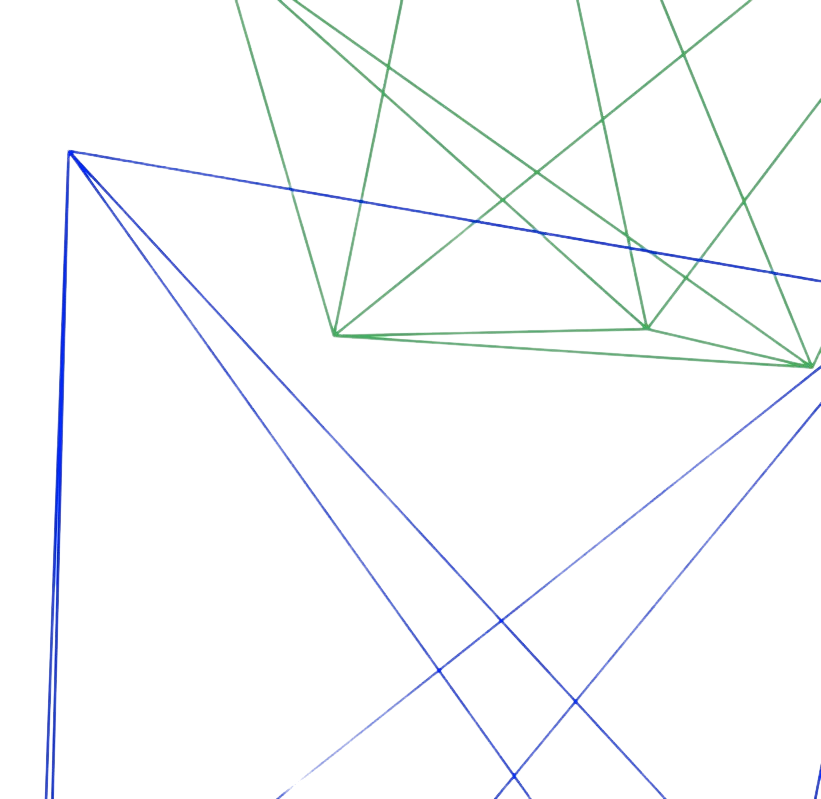
\includegraphics[width=0.5\paperwidth,height=\paperheight]{/root/.config/latex-utils/logos/invert1.png}};

        \node[opacity=0.07,inner sep=0pt, anchor=north west] at (current page.north west){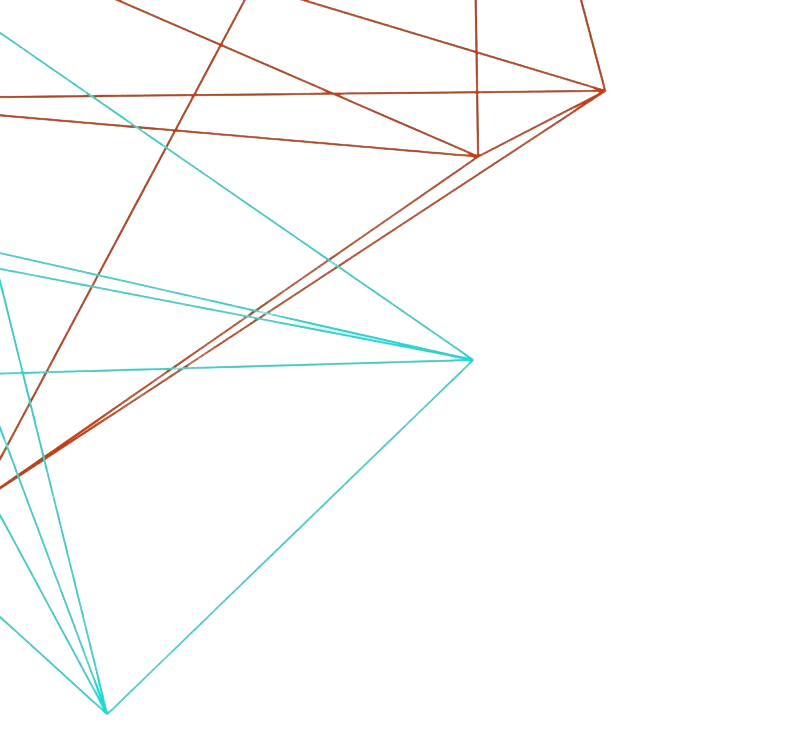
\includegraphics[width=0.5\paperwidth,height=0.5\paperheight]{/root/.config/latex-utils/logos/invert3.png}};




        \node at (page cs:0,0.345) {\Large\textsc{High School Observation and Learning Internship}};
        \node at (page cs:0,0.875) {\Large\bfseries\textsc{Observation Internship}};
        \node at (page cs:0,0.925) {\LARGE\bfseries\textsc{Lycée Français de Barcelone}};

        \node at (page cs:0.5,0) {\Large\textsc{Cyril Lescure - Pedagogical Tutor}};








        %\node[opacity=0.15, inner sep=0pt, anchor=south west] at (current page.south west){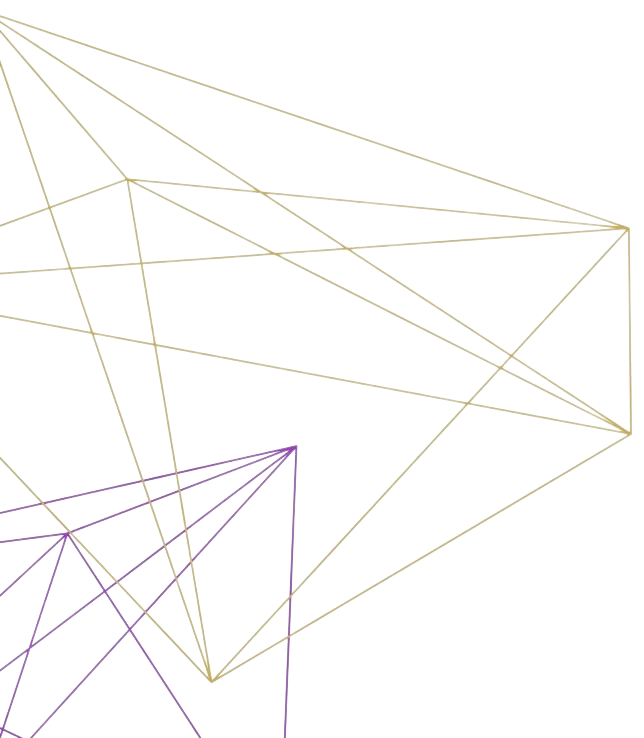
\includegraphics[width=0.5\paperwidth,height=0.5\paperheight]{/root/.config/latex-utils/logos/invert2.png}};

        \node at (page cs:0,0.5) {\fontsize{28}{28.8}\textbf{\ctoptitle}};
        \node at (page cs:0,0.425) {\fontsize{28}{28.8}\textbf{\ctitle}};
        \draw (page cs:0.5,0.375) -- (page cs:-0.5,0.375);
        \node at (page cs:0,0.245) {\LARGE\textsc{\cautor}};
        \node at (page cs:0,0.310) {\Large\textsc{03.06.2019 - 07.06.2019}};


    \end{tikzpicture}
\end{titlepage}


\newgeometry{width=18.625cm, bottom=2cm, top=2cm}

\tikz[remember picture, overlay] \node[opacity=0.3,inner sep=0pt, anchor=north east] at (current page.north east){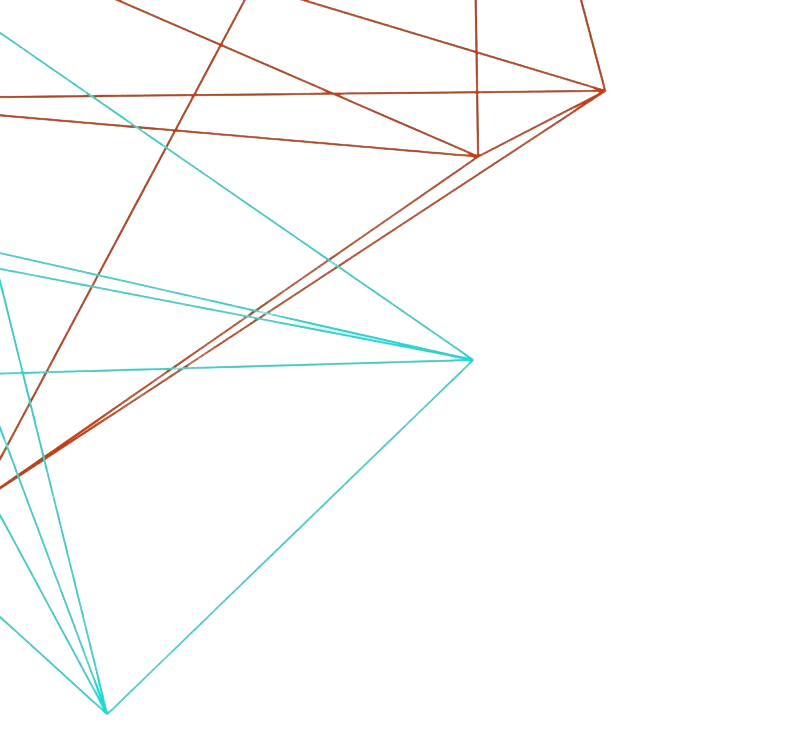
\includegraphics[angle=-90,origin=c,width=0.5\paperheight,height=0.5\paperwidth]{/root/.config/latex-utils/logos/invert3.png}};
\tikz[remember picture,overlay] \node[opacity=0.3,inner sep=0pt, anchor=south east] at (current page.south east){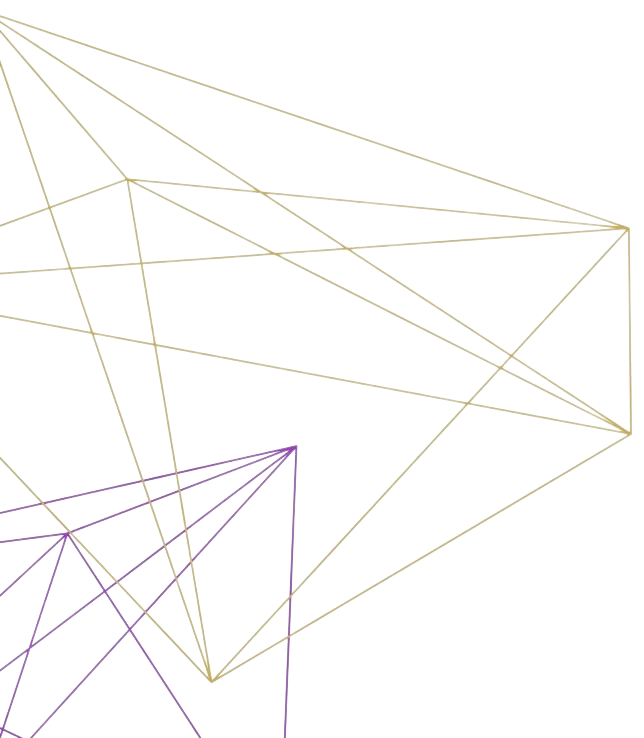
\includegraphics[angle=90,width=0.5\paperwidth,height=0.5\paperheight]{/root/.config/latex-utils/logos/invert2.png}};

\tableofcontents




    
    \newpage

     \section*{Wave propagation in a fiber}

     We begin with the relationships: 
     \linecenter{\hfill$\ds{\vv{D}=\varepsilon_0 \vv{E}+\vv{P}}$ and $\ds{\vv{B}=\mu_0 \vv{H}}$\hfill(with $\ds{\vv{P}=\varepsilon_0 \chi_{ij} \vv{E}}$ and $\ds{\varepsilon_{ij}=1+\chi_{ij}}$ )(1.1)}
     Assuming that the dielectric waveguide is source free and in absence of ferromagnetic materials: 
     \linecenter{$\ds{\vv{\nabla}\cdot \vv{D}= 0}\qquad$ and $\qquad\ds{\vv{\nabla}\times \vv{B}=0}$}

     The electric field described in complex notation is $\ds{\vv{E} =\frac{1}{2}\left[ E_0 e^{i(\omega t-\beta z)} + E_0 e^{-i(\omega t-\beta z)} \right] }$ \hfill(1.2)
     
     Under Maxwell's equations : $\ds{\vv{\nabla}\times \vv{E}=- \frac{\partial \vv{B}}{\partial t}}$ and $\ds{\vv{\nabla} \times  \vv{H}= \frac{\partial \vv{D}}{\partial t} + \vv{J}  }$ \hfill(although $\ds{\vv{J}=0}$)
     
     We then get $\ds{\vv{\nabla } \times  \vv{H} = \frac{\partial }{\partial t} \left( \varepsilon_0 \vv{E}+\vv{P} \right)  }$ 

     Taking the curl of the electric field, we get: 
     \linecenter{\hfill $\ds{\nabla^2 \vv{E} = \mu_0\varepsilon_0 \frac{\partial^{2} \vv{E}}{\partial t^{2}} +\mu_0 \frac{\partial^{2} \vv{P}}{\partial t^{2}} = \mu_0 \varepsilon_0(1+\chi_{ij}) \frac{\partial^{2} \vv{E}}{\partial t^{2}} = \boxed{\mu_0\varepsilon_0\varepsilon_{ij}\frac{\partial^{2} \vv{E}}{\partial t^{2}} }    }$ \hfill(1.3)}

      \subsection*{Wave guides}

      We now hav to introduce guided modes of the optical fiber into the wave equation. Modes are described by a summation of $\ds{l}$ transverse guided modes with amplitude $\ds{A_{\mu}(z)}$, for the core, and a continuum of radiation modes of amplitudes $\ds{A_{\rho}(z)}$, in the cladding due to the large size of the cladding. Each has its own propagation constants $\ds{\beta_{\mu}}$ and $\ds{\beta_{\rho}}$ respectively. 
      
        The corresponding transverse electric field is: 
        \linecenter{\hfill $\ds{\vv{E_t}= \frac{1}{2} \sum_{\mu=1}^{l} \left[ A_\mu(z)\xi_{\mu t} e^{i(\omega t - \beta_\mu z)} + cc \right] + \sum_{\mu=1}^{l} \int\limits_{\rho = 0}^{\rho=\infty} A_\rho(z) \xi_{\rho t} e^{i(\omega t -\beta_\rho z)}  \,d \rho   }$\hfill (1.4)}
        Where $\ds{\xi_{\mu t}}$ and $\ds{\xi_{\rho t}}$ are the transverse field profiles of the guided and radiation modes.
        The sum of radiation modes takes into account the TE, TM, HE and EH modes. And the subscript $\ds{t}$ implicitly includes the polarisation.

        Orthogonality between field distributionf are ensured by the relationship: 
        \linecenter{\hfill $\ds{\frac{1}{2}\int\limits_{-\infty}^{\infty} \int\limits_{-\infty}^{\infty} \left[ \xi_{\mu t} \times  \xi_{\nu t}^*  \right]\cdot \hat{z}   \,d x   \,d y = \frac{1}{2} \frac{\beta_\mu}{\omega\mu_0} \int\limits_{-\infty}^{\infty} \int\limits_{-\infty}^{\infty} \xi_{\mu t} \xi_{\nu t}^* \,d x   \,d y = \delta_{\mu \nu} = \begin{cases}
            1 & \text{if } \mu = \nu\\
            0 & \text{if } \mu \neq \nu 
        \end{cases} }$\hfill (1.5)}

        The mode fields in the core are J-Bessel functions and for the cladding they are K-Bessel functions. In the general case the solutions are two sets of orthogonally polarized modes. The transverse fields for the $\ds{\mu}$-th x-polarised mode satisfying (1.3) along with cladding are : 
        \linecenter{\hfill$\ds{\xi_x = C_\mu J_\mu (u \frac{r}{a}) \begin{pmatrix}
            cos(\mu \phi)\\
            sin(\mu \phi)
        \end{pmatrix} 
        }\qquad$ and $\qquad\ds{\xi_x = C_\mu \frac{J_\mu(\mu)}{\kappa_\mu(w)} \kappa_\mu (w \frac{r}{a}) \begin{pmatrix}
            \cos (\mu \phi)\\
            \sin (\mu \phi) 
        \end{pmatrix} 
        }$ \hfill (1.6)} 

        Where ${u = \frac{2\pi a}{\lambda} \sqrt{n_{core}^2-n_{clad}^2}  }$ and ${w = \frac{2\pi a}{\lambda} \sqrt{n_{eff}^2 - n_{cladd}^2} }$, $\ds{n_{eff}}$ is the is the effective index of the mode expressed as : ${n_{eff}= n_{cladd} \left[ \frac{n_{eff}^2-n_{cladd}^2}{n_{core}^2-n_{eff}^2} \frac{n_{core}-n_{cladd}}{n_{cladd}} +1 \right] }$ 
        
        When assuming only one polarisation then $\ds{\xi_y} =0$
        
        Matching the fields at the core-cladding boundary results in waveguide characteristic eigenvalue equation which may be solved to calculated the propagation constants of the modes: 
        \linecenter{\hfill$\ds{\boxed{u \frac{J_{\mu\pm 1}(u)}{J_\mu(u)}=w \frac{K_{\mu\pm 1}(w)}{K_{\mu}(w)}}}$\hfill (1.7)}

         \section*{Couple mode theory}

         The waveguide modes satisfying the unperturbed wave (1.3) are described by (1.6). In order to derive the couple-mode equations we must include effects of the perturbation, assuming that the modes of the unperturbed waveguide remains unchanged. the mode-coupling is forced by the perturbation as described mathematically for linearised evolution: 
         \linecenter{$\ds{i\tilde{u}t +L \tilde{u} = -iu_{0\tau} + F(u_0,x,t)}$}
         Where $\ds{\tilde{u}}$ are the modes due to the perturbation, $\ds{u_{0\tau}}$ is the slow evolution mode,\\ ${u(x,t,\tau)=\sum_{n=1}^{\infty} a_n(\tau)v_n(x)\exp(i\lambda_nt)}$, and $\ds{F(u_0,x,t)}$ is the perturbation. Thus if $\ds{F(u_0,x,t)}$ is zero then there is no slow evolution of mode parameters $\frac{d\,a_n}{d\tau} = 0$.    

         We first begin with the wave equation : ${\nabla^2  \vv{E} = \mu_0\varepsilon_0 \frac{\partial^{2} \vv{E}}{\partial t^{2}} + \frac{\partial^{2} \vv{P}}{\partial t^{2}}   }$
         We assume that wave propagation takes places in a perturbed system with a dielectric grating such that the total polarization response can be separated into two terms, the unperturbed and the perturbed polarization as: 
         \linecenter{$\ds{\vv{P} = \vv{P}_{unperturbed} + \vv{P}_{grating}} \qquad$ where $\qquad\ds{\vv{P}_{unperturbed}=\varepsilon_0\chi \vv{E_\mu}}$}

         The wave equation then becomes : $\ds{\nabla^2E_{\mu t}= \mu_0\varepsilon_0 \frac{\partial^{2} E_{\mu t}}{\partial t^{2}} + \mu_0 \frac{\partial^{2} }{\partial t^{2}}  P_{grading,\mu}}$ \hfill (2.1)
         
         For the moment, the nature of the perturbed polarization, which is driven by the propagating electric field and is due to the response of the grating, is a detail which we'll include later. 

         Reinserting the modes described in (1.4) into our readapted wave equation yields:
          \begin{multline*}
            \nabla^2 \left[ \frac{1}{2} \sum_{\mu=1}^{l} \left[ A_\mu(z)\xi_{\mu t} e^{i(\omega t - \beta_\mu z)} + cc \right] + \int\limits_{\rho = 0}^{\rho=\infty} A_\rho(z) \xi_{\rho t} e^{i(\omega t -\beta_\rho z)}  \,d \rho \right]\\ -\mu_0\varepsilon_0\varepsilon_r \frac{\partial^{2} }{\partial t^{2}} \left[ \frac{1}{2} \sum_{\mu=1}^{l} \left[ A_\mu(z)\xi_{\mu t}e^{i(\omega t -\beta_\mu z)} \right] + \sum_{}^{} \int\limits_{\rho=-\infty}^{\rho=\infty} A_\rho(z)\xi_{\rho t} e^{i(\omega t-\beta_\rho z)} \,d\rho  \right]\qquad\text{(2.2)}\\ = \mu_0 \frac{\partial^{2} }{\partial t^{2}} P_{grating,\mu}
         \end{multline*}

        If we ignore for the moment the mode coupling to the radiation modes, the left hand side of the equation can be expanded. Considering weak coupling we can simplify the equation by applying the slowly varying envelope approximation. This requires : $\frac{\partial^{2} A_\mu}{\partial z^{2}} \ll \beta_\mu \frac{\partial A_\mu}{\partial z}  $
        
        This way: $\ds{\nabla ^2 E_t = \frac{1}{2} \sum_{\mu=1}^{\infty}\left[ -2i\beta_\mu \frac{\partial A_\mu}{\partial z} \xi_{\mu t}e^{i(\omega t -\beta_\mu z)} -\beta_{\mu}^2A_\mu \xi_{\mu t} e^{i(\omega t - \beta_\mu z)}+ cc \right] }$ \hfill (2.3) 

        Expanding the second term of the left hand side of (2.2) we can note that $\omega^2\mu_0\varepsilon_0\varepsilon_r = \beta_{\mu}^2$ which allows us to cancel a large term in the equation and simplify it to: 
        \linecenter{$\ds{\sum_{\mu=1}^{l} -i\beta_\mu \frac{\partial A_\mu}{\partial z}\xi_{\mu t}e^{i(\omega t - \beta_\mu z)} +cc } = \mu_0\frac{\partial^{2} }{\partial t^{2}} P_{grating,t}$}
        When mutliplying by $\xi_{\mu t}^{*}$ and integrating of the wave-guide cross-section* leads to : 
        \linecenter{$\ds{\sum_{\mu=1}^{l} \int\limits_{-\infty}^{\infty} \int\limits_{-\infty}^{\infty} -2i\omega\mu_0 \frac{\partial A_\mu}{\partial z}\xi_{\mu t}\xi_{\mu t}^{*} e^{i(\omega t- \beta_\mu z)} + cc\,dx \,dy  = \int\limits_{-\infty}^{\infty}\int\limits_{-\infty}^{\infty} \mu_0 \frac{\partial^{2} }{\partial t^{2}} P_{grating,t} \xi_{\mu t}^{*} \,d x   \,d y  }$}

        by using orthogonality relation ship from (1.5) we can simplify the equation to: 
        \linecenter{\hfill$\ds{\boxed{\sum_{\mu=1}^{l} -2i\omega\mu_0 \frac{\partial A_\mu}{\partial z}e^{i(\omega t- \beta_\mu z)} + cc = \int\limits_{-\infty}^{\infty}\int\limits_{-\infty}^{\infty} \mu_0 \frac{\partial^{2} }{\partial t^{2}} P_{grating,t} \xi_{\mu t}^{*} \,d x   \,d y  }}$\hfill (2.4)}

        This is the fundamental wave propagation equationwhich describes coupling of modes. This applies to backwards and forwards propagating modes. The total transverse field can be described  as the sum of both, not necessarily composed of the same mode order: 
        \linecenter{\hfill$\ds{E_t = \frac{1}{2} A_{\nu}\xi_{\nu t}e^{i(\omega t - \beta_\nu z)} +cc + \frac{1}{2} B_\mu\xi_{\mu t}e^{i(\omega t +\beta_{\mu} t)} + cc}$\hfill (2.5)}

        The modes of the waveguide form an orthogonal set which will not couple unless there is a perturbation, using (2.5) and (2.4) yields: 
        
       \linecenter{\hfill$\ds{\frac{\partial A_\nu}{\partial z}e^{i(\omega t-\beta_\nu z)}  + cc- \frac{\partial \beta_\mu}{\partial z} e^{i(\omega t + \beta_\mu z)} + cc} = \frac{i}{2\omega} \int\limits_{-\infty}^{\infty} \int\limits_{-\infty}^{\infty} \frac{\partial^{2} }{\partial t^{2}} P_{grating,t}\xi_{\mu,\nu t}^{*} \,d x  \,d y $\hfill (2.6)}

        \subsection*{Spatially periodic refractive index modulation}

        In a medium where dielectric constant varies periodically along the wave propagation direction, the total polarization can be defined by the perturbed permitivity $\Delta\varepsilon(z)$ and applied field as : $P=\varepsilon_0\left[ \varepsilon_r -1+\Delta\varepsilon(z) \right] E_\mu \qquad$ (2.7)

        The constitutive relation between the permitivity of a material and the refractive index $n$ results in the modulation index being derived from $n^2 = \varepsilon_r$ so that : $\left[ n+ \delta n(z) \right]^2  = \varepsilon_r +\Delta\varepsilon_r(z)$ \hfill (2.8)

        Assuming the perturbation to be a small fraction of the refractive index it follows that $\Delta\varepsilon(z) \approx 2n\delta n(z)$. Defining the refractive index modulation as $\delta n(z)= \overline{\Delta n}\left( 1+ \frac{\nu}{2} \exp (i(\frac{2\pi N}{\Lambda}z -\phi(z))+cc \right)  \qquad$ (2.9). Where $\overline{\Delta n}$ is the average refractive index over a grating period, and $\nu$ is the visibility of the fringes. An arbitrary spatially varying phase $\phi(z)$ was also included and  $N$ is an integer signifying the order of the harmonics.
        
        The period averaged change in the refractive index has to be taken into account since it altres the refractive index $n_{eff}$ of  a mode combining then (2.7) and (2.8) to the expression of polarization we find: 
        \linecenter{$\ds{P = \varepsilon_0\left[ n^2-2+2n \overline{\Delta n}\left( 1+ \frac{\nu}{2} e^{i(\frac{2\pi N}{\Lambda}z+\phi(z))+cc} \right)  \right] E_\mu }$}

        Defining the modulation amplitude by incorporating visibility ($\Delta n = \nu \overline{\Delta n}$), is given as: 
        \linecenter{$\delta n(z) = 2n \left[ \overline{\Delta n} + \frac{\Delta n}{2} e^{i( \frac{2\pi N}{\Lambda} z +\phi(z))+cc} \right] \qquad $ (2.10)}

        The described UV-undiced refractive index change due to grating written into the fiber care as shown in figure 2.1 for index modulation of a uniform grating. Note that in average, index is constant in spite of changes to the visibility even though it remains a function of $\delta n$

        %Fig

        The perturbed polarization can now be related to the refractive index change as given in (2.10), therfore: 
        \linecenter{\hfill$\ds{\boxed{P_{pert} = 2n\varepsilon_0\left( \overline{\Delta n} + \frac{\Delta n}{2} e^{i(\frac{2\pi N}{\lambda}+ \phi(z))} +cc \right)E_\mu }}$\hfill  (2.11)} 

        Using the expression found in (2.6) results in:\footnotesize{ 
         \begin{multline*}
           \frac{\partial A_\nu}{\partial z} e^{i(\omega t - \beta_\nu z)} + cc - \frac{\partial \beta_\mu}{\partial z} e^{i(\omega t + \beta_\mu z)} + cc 
            =  \frac{i}{2\omega} \int\limits_{-\infty}^{\infty} \int\limits_{-\infty}^{\infty} \frac{\partial^{2} }{\partial t^{2}} \left[ \varepsilon_0\delta n\left( A_\nu e^{i(\omega t-\beta_\nu z) \xi_{\nu t}} + B_\mu e^{i(\omega t + \beta _\mu z)}  \xi_{\mu t} \right) \right] \xi_{\mu,\nu t}^*  \,dx \,dy\\
           =-in\omega\varepsilon_0A_\nu \int\limits_{-\infty}^{\infty} \int\limits_{-\infty}^{\infty} \left(\overline{\Delta n} + \frac{\Delta n}{2}e^{i(\frac{2\pi N}{\Lambda}z+\phi(z))} +cc \right)\xi_{\nu t} e^{i(\omega t-\beta_{\nu}z)}\xi_{\mu, \nu t}^*  \,dx \,dy\\ 
           - in\omega\varepsilon_0B_{\mu} \int\limits_{-\infty}^{\infty} \int\limits_{-\infty}^{\infty} \left(\overline{\Delta n}+\frac{\Delta n}{2}e^{i(-\frac{2\pi n}{\Lambda}z -\phi(z))} +cc\right) \xi_{\mu t}e^{i(\omega t +\beta_\mu z)}\xi_{\mu,\nu t}^* \,dx  \,dy + cc  
        \end{multline*} }

         \begin{multline*}
            = -in\omega\varepsilon_0A_\nu e^{i(\omega t -\beta_\nu z)} \int\limits_{-\infty}^{\infty} \int\limits_{-\infty}^{\infty} \overline{\Delta n }\xi_{\nu t}\xi_{\mu,\nu t}^* \,dx  \,dy - in\omega\varepsilon_0B_\mu e^{i(\omega t + (\beta_\mu - \frac{2\pi n}{\Lambda})z+\phi(z))} \int\limits_{-\infty}^{\infty} \int\limits_{-\infty}^{\infty} \frac{\Delta n}{2}\xi_{\mu t}\xi_{\mu,\nu t}^* \,dx  \,dy + cc\\
            -in\omega\varepsilon_0B_\mu e^{i(\omega t-\beta_\mu z)}\int\limits_{-\infty}^{\infty} \int\limits_{-\infty}^{\infty} \overline{\Delta n}\xi_{\mu t}\xi_{\mu,\nu t}^* \,dx  \,dy - in\omega\varepsilon_0A_\nu e^{i(\omega t+(\frac{2\pi N}{\Lambda}-\beta_\nu)z+\phi(z))} \int\limits_{-\infty}^{\infty} \int\limits_{-\infty}^{\infty} \frac{\Delta n}{2}\xi_{\nu t}\xi_{\mu, \nu t}^* \,dx  \,dy +cc 
        \end{multline*}

        Or in other terms:
        \begin{empheq}[box=\fbox]{align}
   \frac{\partial A_\nu}{\partial z} e^{i(\omega t-\beta_\nu z)}+cc = -in\omega\varepsilon_0A_\nu e^{i(\omega t-\beta_\nu z)}\int\limits_{-\infty}^{\infty} \int\limits_{-\infty}^{\infty} \overline{\Delta n}\xi_{\nu t}\xi_{\mu,\nu t}^* \,dx  \,dy - in\omega\varepsilon_0B_\mu e^{i(\omega t + (\beta_\mu +\frac{2\pi N}{\Lambda})z +\phi(z))}\int\limits_{-\infty}^{\infty} \int\limits_{-\infty}^{\infty} \frac{\Delta n}{2}\xi_{\mu t}\xi_{\mu, \nu t}^* \,dx  \,dy +cc \\
       \frac{\partial B_\mu}{\partial z} e^{i(\omega t +\beta_\mu z)}+ cc = in\omega\varepsilon_0B_\mu e^{i(\omega t+\beta_\mu z)} \int\limits_{-\infty}^{\infty} \int\limits_{-\infty}^{\infty} \overline{\Delta n}\xi_{\mu t} \xi_{\mu,\nu t}^*  \,dx \,dy +in\omega\varepsilon_0A_\nu e^{i(\omega t +(\frac{2\pi N}{\Lambda}-\beta_\nu)z+\phi(z))}\int\limits_{-\infty}^{\infty} \int\limits_{-\infty}^{\infty} \frac{\Delta n}{2}\xi_{\nu t}\xi_{\mu, \nu t}^* \,dx  \,dy +cc 
        \end{empheq}

        Two aspects must be taken into account :
         \begin{items}{-15pt}{-15pt}
            \item Conservation of mementum: requires that the phase constants on the left hand side and the right hand side to be identical which influences the coupling between copropagating or counterpropagating modes.
            \item The overlap integral of the index modulation profile and mode fields which determine the strength of the mode interaction.
        \end{items}
        First we'll consider the phase matching condition : $\ds{\beta_\rho=\frac{2 \pi N}{\Lambda}\pm \beta_\nu}$ 
        
         \subsection*{Phase matching}

         From the phase factor given previously, the resultant $\eta_\rho$ is the phase constant of the induced polarization. This is the propagation constant of a bound wave generated by the polarization response of the material due to the presence of sources. For there to be any significant transfer of energy from the driving field amplitude $A_\nu$ to the generated field on the left hand side of (4.7), the generated and the polarization waves remain in phase over an significant distance : $\beta_\mu = \beta_\rho$ (5.1)
         
         %fig

         The polarization wave grows in synchrony with the driving field. The radiating dipoles are shown to be spatially distributed with  aperiod of $\Lambda$ allowing radiated wave to remain in phase with the driving field. This applies to guided or radiating mode coupling.

         Equations (5.1) then describes the phase-matching condition, where a phase mismatch $\Delta \beta$ is referred to as a detuning: $\Delta\beta=\beta_\mu \pm \beta_\nu - \frac{2 \pi N}{\Lambda}$.

         If $A_\nu$ and $B_\mu$ are counterpropagating then the phase matching condition becomes $\Delta\beta=\beta_\mu+\beta_\nu-\frac{2\pi N }{\Lambda}= 0$.
         For copropagating modes the condition becomes $\Delta\beta=\beta_\mu-\beta_\nu-\frac{2\pi N}{\Lambda}=0$.
         Identical relationships apply for radiation mode phase-matching.
         
          \subsection*{Mode symmetry and overlap integral}

          Equation (2.2) suggest that only modes with a same order mode will have a non-zero overlap. However, the presence of non-symmetric index modulation can alter the results allowing modes of different order to overlap.

          The reason for this is the non-uniform transverse distribution of sources giving rise to a polarization wave that has allowed an od symmetry. This is displayed in the figure 6.1: a driving fundamental mode interacts with a modulated permitivity that has uniform transverse profile. 

          %fig

          Examining the transverse overlap on the left half of fthe core we find that it should be the same as the right side, however they are of opposite sign, hence a zero total overlap. This is broken when the index modulation profile is non-uniform inside the core, since the magnitude of the overlap is no longer the same on both sides. Thus a polarisation wave exist with a symmetry (and mode order) different from the driving mode, exhange of energy is then allowed to happen.

          The consequence of the asymmetric index perturbation is now apreciated in (4.7):

          
         \linecenter{$\ds{\frac{\partial A_\nu}{\partial z} e^{i(\omega t-\beta_\nu z)}+cc = -in\omega\varepsilon_0A\nu e^{i(\omega t- \beta_\nu z)}\int\limits_{-\infty}^{\infty} \int\limits_{-\infty}^{\infty} \overline{\Delta n}\xi_{\nu t}\xi_{\mu,\nu t}^* \,dx  \,dy -in\omega\varepsilon_0 B_\mu e^{i(\omega t +(\beta_\mu -\frac{2\pi N}{\Lambda})z-\phi(z))}\int\limits_{-\infty}^{\infty} \int\limits_{-\infty}^{\infty} \frac{\Delta n}{2}\xi_{\mu t}\xi_{\mu,\nu t}^* \,dx  \,dy + cc }$} 
         \linecenter{$\ds{\frac{\partial B_\mu}{\partial z} e^{i(\omega t +\beta_\mu z)}+cc = i n \omega\varepsilon_0 \beta_\mu e^{i(\omega t +\beta_\mu z)}\int\limits_{-\infty}^{\infty} \int\limits_{-\infty}^{\infty} \overline{\Delta n}\xi_{\mu t}\xi_{\mu,\nu t}^* \,dx  \,dy +in\omega\varepsilon_0 A_\nu e^{i(\omega t +(\frac{2 \pi N}{\Lambda}-\beta_\nu)z+\phi(z)}  \int\limits_{-\infty}^{\infty} \int\limits_{-\infty}^{\infty} \frac{\Delta n}{2}\xi_{\nu t}\xi_{\mu,\nu t}^* \,dx  \,dy +cc }$}

         The integration where the driving field $\xi_{\mu t}$ and the polarization field $\xi_{\nu t}$ along with the asymetric index modulation are non-zero for dissimilar mode orders $\mu=\nu$. The magnitude of the overlap for a particular mode combination will depend on exact details of the pertubation profile.

          \subsection*{Periodic nonsinusoidal index modulation}

          For non-sinusoidal but periodic functoins we can apply the Fourier transform to decompose the profile into a sum of sinusoidal functions, we can then expand $\delta n$ as : 
          \linecenter{$\ds{\delta n(z) = 2n\left[ \overline{\Delta n} + \frac{\Delta n}{2} \sum_{N=-\infty}^{N=\infty} \alpha_N e^{i(\frac{2\pi N}{\Lambda}z +\phi(z))}+cc \right] }$}
          \hfill (where $\alpha_N$ is the Fourier amplitude coefficient)

         \subsection*{Coupling of counter propagating guided modes}

         For a general approach, dissimilar modes are considered for the counterpropagating mode phase-matching condition. 
         \linecenter{$\ds{\frac{\partial B_\mu}{\partial z} e^{i(\omega t-\beta_\mu z)}=in\omega\varepsilon_0B_\mu e^{i(\omega t +\beta_\mu z)}\int\limits_{-\infty}^{\infty} \int\limits_{-\infty}^{\infty} \overline{\Delta n}\xi_{\mu t}\xi_{\mu,\nu t}^* \,dx  \,dy + in\omega\varepsilon_0A_{\nu}e^{i(\omega t+ (\frac{2 \pi N}{\Lambda}-\beta_\nu)z + \phi(z)}  \int\limits_{-\infty}^{\infty} \int\limits_{-\infty}^{\infty} \frac{\Delta n}{2}\xi_{_\nu t}\xi_{\mu,\nu t}^* \,dx  \,dy +cc }$}

         Which becomes: $\ds{\frac{\partial B_\mu}{\partial z} =in\omega\varepsilon_0B_\mu \int\limits_{-\infty}^{\infty} \int\limits_{-\infty}^{\infty} \overline{\Delta n}\xi_{\mu t}\xi_{\mu,\nu t}^* \,dx  \,dy +in\omega\varepsilon_0A_\nu e^{i((\frac{2\pi N}{\Lambda}-\beta_\nu-\beta_\mu)z+\phi(z))} \int\limits_{-\infty}^{\infty} \int\limits_{-\infty}^{\infty} \frac{\Delta n}{2}\xi_{\nu t}\xi_{\mu,\nu t}^* \,dx  \,dy +cc }$

         This is further simplified as the couple-mode equations : 
         \linecenter{$\ds{i\frac{\partial B_\mu}{\partial z} = n\omega\varepsilon_0B\mu \int\limits_{-\infty}^{\infty} \int\limits_{-\infty}^{\infty} \overline{\Delta n}\xi_{\mu t}\xi_{\mu,\nu t} \,dx \,dy + n\omega\varepsilon_0A_\nu\int\limits_{-\infty}^{\infty} \int\limits_{-\infty}^{\infty} \frac{\Delta n}{2}\xi_{\nu t}\xi_{\mu,\nu t}  \,dx  \,dy\  e^{i((\frac{2\pi N}{\Lambda}-\beta_\nu-\beta_\mu)z+\phi(z))} }$} 
         \linecenter{$\ds{-i\frac{\partial A_\nu}{\partial z} =n\omega\varepsilon_0A_\nu \int\limits_{-\infty}^{\infty} \int\limits_{-\infty}^{\infty} \overline{\Delta n}\xi_{\nu t}\xi_{\nu t}^* \,dx  \,dy + n\omega\varepsilon_0B_\nu \int\limits_{-\infty}^{\infty} \int\limits_{-\infty}^{\infty} \frac{\Delta n}{2}\xi_{\mu t}\xi_{\nu t}^* \,dx  \,dy\  e^{i((\beta_\nu+\beta_\mu-\frac{2\pi N}{\Lambda})z -\phi(z))}}$}

         To find a solution to the couple-mode equation the following substitution can be made for backward and forward modes: 
         \linecenter{$\ds{R=A_{\nu}e^{-\frac{1}{2}i(\Delta\beta z-\phi(z))}\qquad}$ and $\ds{\qquad S=B_\mu e^{\frac{1}{2}i(\Delta\beta z-\phi(z))}}$ }

         Differentiating the substitution and inserting into the couple-mode equations yields: 
         \linecenter{$\ds{\frac{d\, R}{d z} +iR\left( K_{dc}+\frac{1}{2}(\Delta\beta-\frac{d\, \phi(z)}{d z} ) \right) =-iSK_{ac}^*\qquad}$ and $\ds{\qquad \frac{d\, S}{d z} -iS\left(K_{dc}+\frac{1}{2}(\Delta\beta -\frac{d\, \phi(z)}{d z} )\right) =iRK_{ac} }$ } 
         \linecenter{\hfill(where$\ds{K_{dc}=\int\limits_{-\infty}^{\infty} \int\limits_{-\infty}^{\infty} \overline{\Delta n}\xi_{\mu t}\xi_{\mu t}^* \,dx  \,dy  }$ and $\ds{K_{ac}=\int\limits_{-\infty}^{\infty} \int\limits_{-\infty}^{\infty} \frac{\Delta n}{2}\xi_{\mu t}\xi_{\nu t}^* \,dx  \,dy }$) }

         $K_{dc}$ influences propagation due to the change in average index of the mode. Any absorption, scatter loss, or gain can be incorporated in the magnitude and sign of the imaginary part of $K_{dc}$.

         There are also 2 additional terms inside the parenthesis: The first term, $\frac{\Delta\beta}{2}$ is the detuning and indicates how rapidly the power is exchanged between radiated fields and the polarisation field. This weighing factor is proportional to the inverse of the distance the field travels in the generated mode. At phase-matching condition, the field couple to the generated wave over an infinite distance. Finally, the rate of change of $\phi(z)$ ingnifies a chirp in the period of the grating and has an effect similar to the detuning. So for uniform grating $\frac{d\, \phi(z)}{d z} =0$ and a visibility of 1, $K_{ac}=\frac{K_{dc}}{2}$

         The couple-mode equations are solved using standard techniques. First the eigenvalues are determined by replacing the differential operator by $\lambda$ and solving the characteristic equation by equaling the characterictic determinant to zero. The resultant eigenvalue equation is in general a polynomial in the eigenvalue $\lambda$. Once eigenvalues are found, the boundary values are applied for uniform grating. We assume that the amplitude of the incident radiation is $R(0)=1$ and $S(L)=0$. The latter condition is satisfied by the fact that the reflected field at the output end of the grating can not exist owing to the absence of the perturbation beyond that region. These conditions result in the following analyticalsolution for the amplitude reflection coefficient: 
         \linecenter{$\ds{\rho=\frac{S(0)}{R(0)}=\frac{-K_{ac}\sin(\alpha L)}{\delta \sin(\alpha L)-i\alpha\cos(\alpha L)}}$ and power coefficient $\ds{ \lvert \rho \rvert^{2} = \frac{\lvert \rho \rvert}{} }$ }

         

         


         

        

         

    
      

         
             

            %\linecenter{\hfill$\ds{\nabla^2 \left[ \frac{1}{2} \sum_{\mu=1}^{l} \left[ A_\mu(z)\xi_{\mu t} e^{i(\omega t - \beta_\mu z)} + cc \right] + \int\limits_{\rho = 0}^{\rho=\infty} A_\rho(z) \xi_{\rho t} e^{i(\omega t -\beta_\rho z)}  \,d \rho \right] = -\mu_0\varepsilon_0\varepsilon_r \frac{\partial^{2} }{\partial t^{2}} \left[ \frac{1}{2} \sum_{n=1}^{\infty} \left[ A_\mu(z)\xi_{\mu t}e^{i(\omega t -\beta_\mu z)} \right]  \right]   }$ \hfill (2.2)}




 
 

\end{document}